\subsection{Opgaver}

\begin{enumerate}
	\item Udregn
	\begin{align*}
	\int_{0}^{\frac{\pi}{4}} \sin(-x) \dd x,&& \int_{0}^{\sqrt[3]{\frac{\pi}{2}}} 3x^2\cos(x^3) \dd x,&& \int_{0}^{\frac{\pi}{6}}\cos(x)\sin^2(x) \dd x
	\end{align*}
	
	
	
	\item Udregn
	\begin{align*}
	\int_0^3 x^2\sqrt{x^3+9}\dd x,&& \int_0^\frac{\pi}{4} \frac{\cos x}{1+\sin x} \dd x,&& \int_0^1 \frac{x}{(1+x^2)^2}\dd x.
	\end{align*}
	
	\item\label{it:bes11} En funktion $f$ siges at være ulige hvis $f(-x)=-f(x)$. Vis at
	\begin{align*}
	\int_{-a}^{a}f(x)\dd x=0,
	\end{align*}
	såfremt $f$ er kontinuert.
	(Hint: Brug variabelskiftet $u=-x$ og Opgave~\ref{it:bes3} til at vise 
	\begin{align*}
	\int_{-a}^{0}f(x)\dd x=-\int_{0}^{a}f(x)\dd x.
	\end{align*}
	Brug efterfølgende Opgave~\ref{it:best2} til at færdiggøre opgaven.)
	
	\item Udregn
	\begin{align*}
	\int_{-\frac{\sqrt{3}}{3}}^{\frac{\sqrt{3}}{3}} (3x^2-1)(x^3-x)^3 \dd x,&& \int_{-1}^{1} \sin(x)e^{\cos(x)}\dd x,&& \int_{-100}^{100} x\abs{x}\dd x.
	\end{align*}
	(Hint: Brug Opgave~\ref{it:bes11})
	
	
	\item\label{it:bes12} En funktion $f$ siges at være lige hvis $f(-x)=f(x)$. Vis at
	\begin{align*}
	\int_{-a}^{a} f(x)\dd x =2\int_{0}^{a}f(x) \dd x,
	\end{align*}
		såfremt $f$ er kontinuert.
	(Hint: Brug variabelskiftet $u=-x$ og Opgave~\ref{it:bes3} til at vise 
	\begin{align*}
	\int_{-a}^{0}f(x)\dd x=\int_{0}^{a}f(x)\dd x.
	\end{align*}
	Brug efterfølgende Opgave~\ref{it:best2} til at færdiggøre opgaven.)
	
	\item Udregn
	\begin{align*}
	\int_{-\sqrt[3]{\frac{\pi}{2}}}^{\sqrt[3]{\frac{\pi}{2}}} 6x^2\cos(x^3) \dd x,&& \frac{1}{2}\int_{-\frac{pi}{6}}^{\frac{\pi}{6}}\cos(x)\sin^2(x) \dd x
	\end{align*}
		(Hint: Brug Opgave~\ref{it:bes12})
	
	\item Lad $f(x)=x^{-2}\sin (\frac{1}{x})$.
	\begin{enumerate}
		\item Vis at $f$ er en ulige funktion.
		\item Bestem en stamfunktion til $f$. 
		\item Integralet 
		\begin{align*}
		\int_{-1}^{1} f(x)\dd x,
		\end{align*}
		er ikke defineret. Hvordan stemmer det overens med resultatet i Opgave~\ref{it:bes11}?
	\end{enumerate} 
	
	\item I Opgave~\ref{it:diff24} blev det vist at
	\begin{align*}
	\int xe^x\dd x=(x-1)e^x+C.
	\end{align*}
	Brug dette til at vise at 
	\begin{align*}
	\int_0^1 e^{\sqrt{x}}\dd x =2.
	\end{align*}
	(Hint: substituer $u=\sqrt{x}$ så variabelskiftet bliver $2u du =dx$.)
	
	\item I Opgave~\ref{it:int21} så vi at 
	\begin{align*}
	\int x\sin x\dd x=\sin x-x\cos x+C.
	\end{align*}
	Brug dette til at vise at 
	\begin{align*}
	\int_0^{\pi^2} \sin\sqrt{x}\dd x =2\pi
	\end{align*}
		(Hint: substituer $u=\sqrt{x}$ så variabelskiftet bliver $2u du =dx$.)
	
	\item I denne opgave vil vi beskrive arealet af en cirkel med vilkårlig radius.
	\begin{enumerate}
		\item Tallet $\pi$ kan defineres som arealet af enhedscirklen. Brug denne definition til at konkludere at
		\begin{align*}
		4\int_0^1 \sqrt{1-x^2}\dd x=\pi.
		\end{align*}
		(Hint: Enhedscirklen er defineret ved $x^2+y^2=1$.)
		\item Brug formlen ovenfor til at vise at arealet af cirklen givet ved $x^2+y^2=r^2$ har areal $A=\pi r^2$.
		(Hint: Brug udregningen
		\begin{align*}
		A=4\int_0^r \sqrt{r^2-x^2}\dd x=4r\int_0^r \sqrt{1-\frac{x^2}{r^2}}\dd x,
		\end{align*}
		og substituer $u=\frac{x}{r}$.)
	\end{enumerate}
	\item\label{it:bes2} En ellipse kan beskrives ved ligningen 
	\begin{align}\label{eq:bes1}
	\frac{x^2}{a^2}+\frac{y^2}{b^2}=1,
	\end{align}
	 hvor betydningen af $a$ og $b$ kan ses i Figur~\ref{fig:bes2}.
			\begin{enumerate}
				\item Vis at hvis $a=b$ så beskriver~\eqref{eq:bes1} en cirkel. 
				\item Brug samme fremgangsmåde som i Opgave~\ref{it:bes2} til at vise at arealet af en ellipse er givet ved $\pi a b$.
				\item Hvordan stemmer dette over ens med at arealet af en cirkel er givet ved $\pi r^2$.
			\end{enumerate}

	\begin{figure}
	\centering
	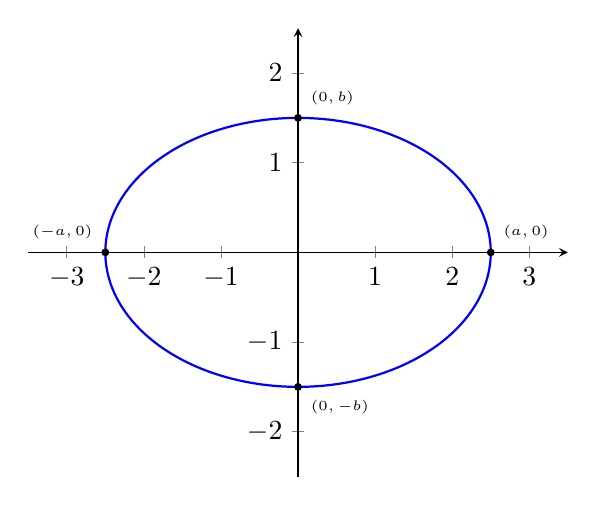
\begin{tikzpicture}
	\begin{axis}[axis x line=center,xmin=-3.5,xmax=3.5,ymin=-2.5,ymax=2.5,axis y line=center]
	\addplot[thick,blue,domain=0:2*pi,samples=300] ({5/2*cos(deg(x))},{3/2*sin(deg(x))});
	\node[fill, circle, inner sep=1pt] at (axis cs:0,3/2) [label=above right: {\tiny$(0,b)$}]{};
	\node[fill, circle, inner sep=1pt] at (axis cs:0,-3/2) [label=below right: {\tiny$(0,-b)$}]{};
	\node[fill, circle, inner sep=1pt] at (axis cs:5/2,0) [label=above right: {\tiny$(a,0)$}]{};
	\node[fill, circle, inner sep=1pt] at (axis cs:-5/2,0) [label=above left: {\tiny$(-a,0)$}]{};
	\end{axis}
	\end{tikzpicture}
	\caption{Opgave~\ref{it:bes2}}
	\label{fig:bes2}
	\end{figure}
	\item Bestem
	\begin{align*}
	 \int_0^\pi x^2\cos x \dd x.
	\end{align*}
	
		\item Bestem integralerne
	\begin{align*}
	\int_0^{\frac{\pi}{2}} x\cos x\dd x,&& \int_0^{\ln 2} x e^{2x} \dd x,&& \int_1^4 3x^2\ln x\dd x.
	\end{align*}
	
		\item Bestem arealet afgrænset af $x$-aksen og grafen for funktionen $f(x)=x^2\sin x$ fra $0$ til $\pi$.
		
			\item Funktionerne $\sin(x)\cos(x)$ og $\frac{1}{2}\sin x$ skærer hinanden i $0$ og $\frac{\pi}{3}$. Hvad er arealet mellem graferne for funktionerne i intervallet givet af deres skæringspunkter?
\end{enumerate}